%========================================================================================
\section{Supporting Information on Chapter 3} \label{Annex_chap3} \begin{refsection}
%========================================================================================

\clearpage

%++++++++++++++++++++++++++++++++++++++++++++++++++++++++++++++++++++++++++++++++++++++++
\begin{figure}[ht]
  \centering
  \begin{minipage}{0.2\textwidth}
    \centering
    
\includegraphics[width=\textwidth]{figures/ies logo.png}
  \end{minipage}
  \hfill
  \begin{minipage}{0.4\textwidth}
    \centering
    
\includegraphics[width=\textwidth]{figures/logo_rptu.png}
  \end{minipage}
  \vspace{5cm}
\end{figure}
%++++++++++++++++++++++++++++++++++++++++++++++++++++++++++++++++++++++++++++++++++++++++

\begin{center} 
\HRule 
\vspace{0.2cm}
\Huge \textbf{Standard Operating Procedure for Field Sampling of Soil for Mycotoxin Analysis}
\vspace{0.2cm}
\HRule 
\end{center}

\vspace{2cm}
\begin{center} 
\LARGE \textit{By} Julius Albert and Katherine  Munoz


\LARGE June 2020
\end{center}

\clearpage



%\renewcommand{\thesection}{}
%\renewcommand{\thesubsection}{}


\noindent\large{\textbf{Scope and Field of Application}}
%----------------------------------------------------------------------------------------


The provided standard operating procedures are designed to assist researchers and practitioners in effectively sampling agricultural soil for the determination of mycotoxin field levels.  Accurately assessing mycotoxin occurrence and distribution within a field requires the utilization of appropriate, reliable, and reproducible sampling techniques. Agricultural soils possess inherent heterogeneity, both across the field and down the soil profile, leading to highly variable mycotoxin levels even on small scales. This inherent variability emphasizes the need for careful sampling to ensure that the collected samples truly represent the occurrence and distribution in the field. When aiming to determine representative mean levels of mycotoxins on a field scale, multiple clusters should be selected in the field. From each cluster, numerous individual samples must be collected at different positions (between plants and inter-row) and depths (topsoil and subsoil) using a fine mesh of sampling points. These samples should be adequately homogenized to obtain pooled samples that accurately represent the respective positions and depths of each cluster. By following these instructions, researchers and practitioners can obtain reliable and representative data on mycotoxin levels in agricultural soils. This information contributes to the development of effective management strategies and supports decision-making in the agricultural sector.

%----------------------------------------------------------------------------------------
\subsection*{Materials}
%----------------------------------------------------------------------------------------

The following materials are required for field sampling:

\begin{itemize}
  \item Appropriate sample container e.g. plastic Bags (minimum 0.5 L) 
  \item Large Spoon
  \item Auger
  \item Large wooden/plastic hammer
  \item Knife
  \item Permanent Marker
  \item Portable Balance
  \item Meterstick
  \item Buckets
  \item Deionized water
\end{itemize}

%----------------------------------------------------------------------------------------
\subsection*{Preliminary Preparation}
%----------------------------------------------------------------------------------------

Before and after sampling, clean the sampling equipment with deionized water to reduce sample carryover and contamination. This includes the auger, buckets, spoon and knife. If necessary, and especially when changing to another field, it is advisable to draw a soil core once and then discard it. In this way, the equipment is pre-rinsed with the new field soil.

%----------------------------------------------------------------------------------------
\subsection*{Soil Sampling Procedure}
%----------------------------------------------------------------------------------------

%++++++++++++++++++++++++++++++++++++++++++++++++++++++++++++++++++++++++++++++++++++++++
\begin{figure}[b!]
\centering
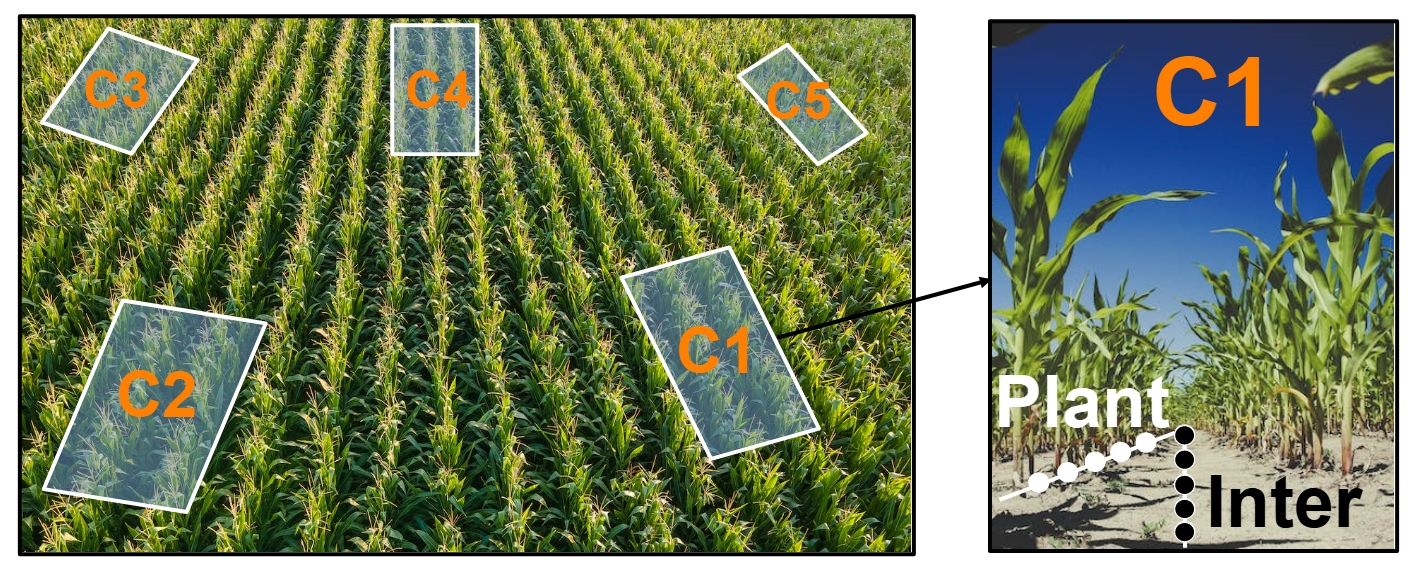
\includegraphics[width=1\textwidth]{figures/sop_soil sampling 1.jpg}
\decoRule
\captionsetup{labelfont=bf, justification=justified, singlelinecheck=false, width=1\textwidth} 
\caption{Scheme for field sampling of soil for mycotoxin analysis. A minimum of 5 clusters are assigned in the field. In each cluster, 5 individual sampling positions are designated between the plants in the planting row ("Plant") and 5 samples are designated in the inter-row ("Inter").}
\label{fig:SOP1}
\end{figure}
%++++++++++++++++++++++++++++++++++++++++++++++++++++++++++++++++++++++++++++++++++++++++

In a first step, a minimum of 5 clusters are assigned in the field and labeled with a unique identifier. Each cluster should consist of a minimum of 10 crop plants. A minimum of 5 individual samples are taken between the plants in the plant row, and an additional 5 sampling points are designated at the same height in the inter-row position (Figure \ref{fig:SOP1}).


Four sampling buckets are provided to collect the individual samples for each combination of position (at-plant and inter-row) and depth (topsoil and subsoil). At each sampling point, the auger is drilled straight into the ground using the sampling hammer to obtain a soil core of approximately 35-40 cm. The soil core is then divided into three sections by making a cut with a knife: 0-15 cm, 15-30 cm, and >30 cm. The last fraction is discarded. The 0-15 cm section is collected in the respective topsoil sampling bucket for each position, while the 15-30 cm section is collected in the respective subsoil sampling bucket (Figure \ref{fig:SOP2}). The individual samples from each position and depth within a cluster are combined in their respective buckets and thoroughly mixed using a spoon. Large rocks and plant materials are to be removed. Approximately 300 g of the homogenized sample is then placed into the corresponding sample bag.

%++++++++++++++++++++++++++++++++++++++++++++++++++++++++++++++++++++++++++++++++++++++++
\begin{figure}[h]
\centering
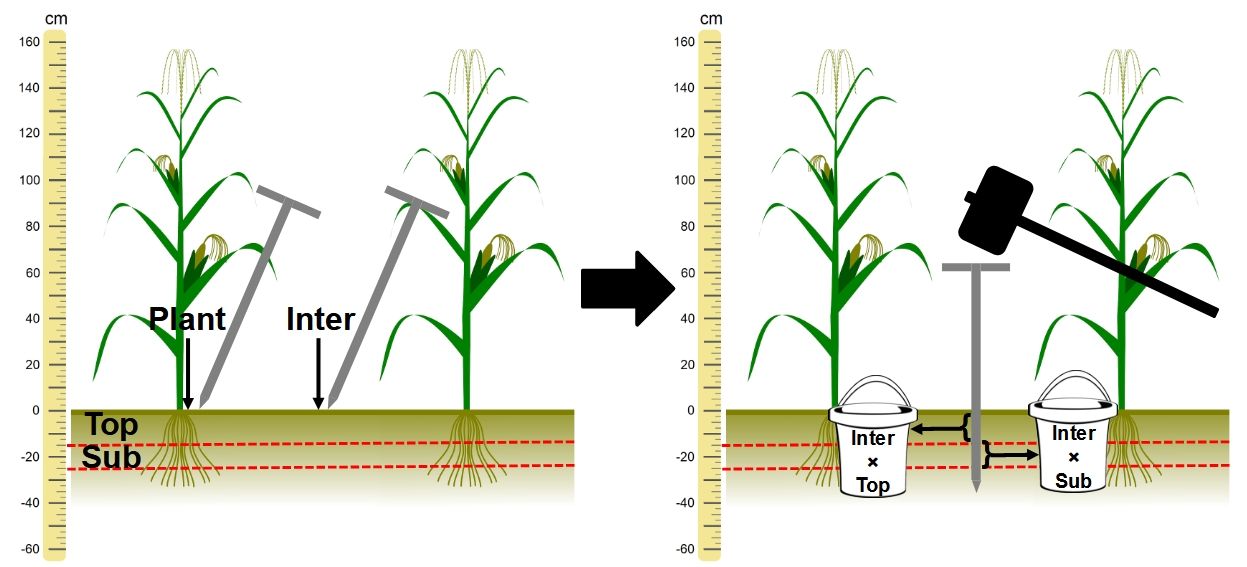
\includegraphics[width=1\textwidth]{figures/sop_soil sampling 2.jpg}
\decoRule
\captionsetup{labelfont=bf, justification=justified, singlelinecheck=false, width=1\textwidth}
\caption{Soil sampling procedure. At each cluster, soil cores are taken at the "Plant" and "Inter" positions using a soil auger. The soil cores are then divided into "upper" (0-15 cm) and "lower" soil layers (15-30 cm). The individual samples for each position and depth are collected in buckets and homogenized by mixing with a spoon to obtain a homogenized composite sample.}
\label{fig:SOP2}
\end{figure}
%++++++++++++++++++++++++++++++++++++++++++++++++++++++++++++++++++++++++++++++++++++++++

%----------------------------------------------------------------------------------------
\subsection*{Packaging, Storage and Transport}
%----------------------------------------------------------------------------------------

To ensure the preservation and integrity of samples during storage or transport, it is important to use appropriate, robust and non-reactive packaging materials, such as plastic or paper bags. This choice of packaging will help protect samples from moisture, pests, spills, and contamination. Since most mycotoxins are susceptible to photolytic and microbial degradation, it is advisable to store samples in a cool, light-protected environment as soon as possible after collection. For short-term storage of a few weeks, a temperature of at least 4 °C is recommended, while for longer-term storage over months, a temperature of at least -20 °C should be maintained.

%----------------------------------------------------------------------------------------
\subsection*{Recording}
%----------------------------------------------------------------------------------------

Each pooled sample should be labeled accordingly. The label should contain the following information:

\begin{itemize}
\item Field number
\item Cluster number
\item Position (At-Plant or Inter-Row)
\item Layer (Topsoil or Subsoil)
\item Date
\end{itemize}

In addition, the following information should be collected during each field sampling and attached to the respective field batch of samples on an information sheet:
\begin{itemize}
\item Name of the collecting institution and personnel
\item Photographs of the field, close-ups of the ground and crop plants
\item Weather conditions
\item Date
\item Start and finish time
\item GPS coordinates
\item Optional: additional field parameters may be recorded, such as treatments.
\end{itemize}

%\setcounter{section}{0}
\clearpage
\end{refsection} % section bibliography
